\documentclass{article}
\usepackage[utf8]{inputenc}
\usepackage{tikz}

\title{Binary soft LDPC decoder}
\author{}
\date{}

\begin{document}

\maketitle

\section{Sparse matrix representation}
Consider a toy-example $m\times n$ parity check matrix:
\begin{equation}
\label{eq:h_binary}
\mathbf{H} = \left[
\begin{array}{ccccc}
0 & 0 & 0 & 1 & 1 \\
0 & 1 & 1 & 0 & 0 \\
1 & 0 & 1 & 0 & 1 \\
1 & 1 & 0 & 1 & 0 \\
\end{array}
\right]
\end{equation}
Each nonzero element of the parity check matrix~(\ref{eq:h_binary}) corresponds to a single message in the Tanner graph. Now let us construct the sparse form of~$\mathbf{H}$. One can do this as follows. For each row one can write the indexes of non-zero elements. As a result, each row or column of~$\mathbf{H}$ is an index array. The length of this array corresponds to the row or column weight ($w_r$ and $w_c$, respectively).
\begin{equation}
\label{eq:h_sparse}
% \left[
\begin{array}{cccccc}
w_c & 2 & 2 & 2 & 2 & 2 \\
 & \downarrow & \downarrow & \downarrow & \downarrow & \downarrow \\
& 2 & 1 & 1 & 0 & 0 \\
& 3 & 3 & 2 & 3 & 2 \\
\end{array}
% \right]
\quad  \quad
% \left[
\begin{array}{ccccc}
w_r & & & \\
2 & \rightarrow & 3 & 4 &   \\
2 & \rightarrow & 1 & 2 &   \\
3 & \rightarrow & 0 & 2 & 4 \\
3 & \rightarrow & 0 & 1 & 3 \\
\end{array}
% \right],
\end{equation}
As a result,~(\ref{eq:h_sparse}) is an equivalent form of $\mathbf{H}$. This form consists of the row or column weight vector and a matrix of indices having the sizes $n \times \max{\left(w_c\right)}$ and $\max{\left(w_r\right) \times m}$ for the first and the second representation. We assume the zero-padding for rows and columns having a weight smaller than the maximum weight.

Representations~(\ref{eq:h_binary}) and ~(\ref{eq:h_sparse}) are equivalent and the first one is column-perspective and the second one is a row-perspective representations (in accordance with arrows direction).

\section{Tanner graph messages indexing}
Each nonzero element of~$\mathbf{H}$ corresponds to a Tanner graph message. The LDPC decoder runs through the messages row-by-row performing the check nodes update first.

The messages are stored in the row-perspective sparse representation~(\ref{eq:h_sparse}). As a result, the message index is a pair of numbers. The first number is a row index in the row-perspective sparse representation matrix ($i$, running from $0$ to $m - 1$. The second number -- column index ( $j$ running from $0$ to $w_r^{(i)} - 1$). As a result, running the check node update involves scanning the messages by iterating $i$ and $j$. 

During the check node update, one gets the following message ordering:

\begin{equation}
\label{eq:msg_idx}
\mathbf{H} = \left[
\begin{array}{ccccc}
\cdot & \cdot & \cdot &     0 &     1 \\
\cdot &     2 &     3 & \cdot & \cdot \\
    4 & \cdot &     5 & \cdot &     6 \\
7 & 8 & \cdot & 9 & \cdot \\
\end{array}
\right]
\end{equation}

Now, let us make the correspondence between message ordering and message indexing (as a pair of numbers described above). One can easily construct the following table.
\begin{equation}
\label{eq:row_indexing}
\begin{array}{cccccccccc}
0      & 1      & 2      & 3      & 4      & 5      & 6      & 7      & 8      & 9      \\
{0 \choose 0} & {0 \choose 1} & {1 \choose 0} & {1 \choose 1} & {2 \choose 0} & {2 \choose 1} & {2 \choose 2} & {3 \choose 0} & {3 \choose 1} & {3 \choose 2} \\
\end{array}
\end{equation}

At the variable node update, one runs through the messages scanning $\mathbf{H}$ column by column. The message order changes in this case to the following one.
\begin{equation}
\label{eq:col_indexing}
\begin{array}{cccccccccc}
4      & 7      & 2      & 8      & 3      & 4      & 0      & 9      & 1      & 6      \\
{0 \choose 0} & {0 \choose 1} & {1 \choose 0} & {1 \choose 1} & {2 \choose 0} & {2 \choose 1} & {3 \choose 0} & {3 \choose 1} & {4 \choose 0} & {4 \choose 1} \\
\end{array}
\end{equation}
To construct the table above, one can scan the matrix~(\ref{eq:msg_idx}) column by column and to use the column-perspective sparse representation of~$\mathbf{H}$~(\ref{eq:h_sparse}).

As one can see, the column-by-column matrix scanning results in the message permutation. The pairs of indices below correspond to the column-perspective sparse representation. At the variable node update, one needs to construct a mapping between index pairs of~(\ref{eq:col_indexing}) and index pairs of~(\ref{eq:row_indexing}). This mapping has been presented in~Fig.~\ref{fig:msg_map}. The ``Index'' corresponds to column-perspective message iteration (during the variable node updates) and ``Value'' corresponds to the message index stored in the row-perspective manner.

\begin{figure}
\centering
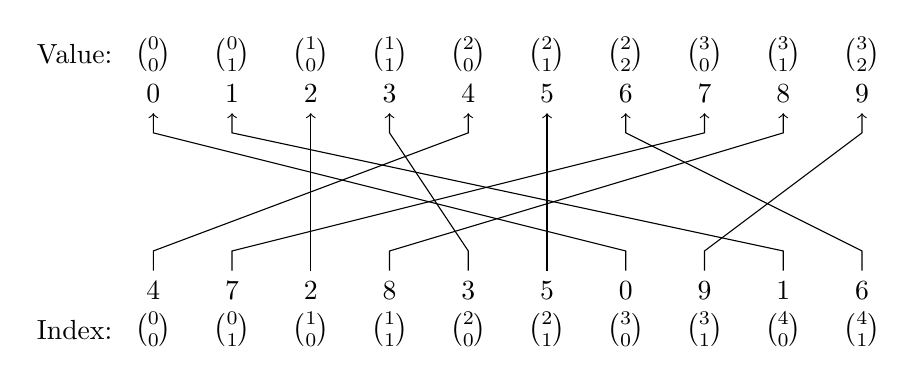
\begin{tikzpicture}
\node () at (0, 4) {${0 \choose 0}$};
\node () at (1, 4) {${0 \choose 1}$};
\node () at (2, 4) {${1 \choose 0}$};
\node () at (3, 4) {${1 \choose 1}$};
\node () at (4, 4) {${2 \choose 0}$};
\node () at (5, 4) {${2 \choose 1}$};
\node () at (6, 4) {${2 \choose 2}$};
\node () at (7, 4) {${3 \choose 0}$};
\node () at (8, 4) {${3 \choose 1}$};
\node () at (9, 4) {${3 \choose 2}$};

\node () at (0, 3.5) {$0$};
\node () at (1, 3.5) {$1$};
\node () at (2, 3.5) {$2$};
\node () at (3, 3.5) {$3$};
\node () at (4, 3.5) {$4$};
\node () at (5, 3.5) {$5$};
\node () at (6, 3.5) {$6$};
\node () at (7, 3.5) {$7$};
\node () at (8, 3.5) {$8$};
\node () at (9, 3.5) {$9$};


\node () at (0, 1) {$4$};
\node () at (1, 1) {$7$};
\node () at (2, 1) {$2$};
\node () at (3, 1) {$8$};
\node () at (4, 1) {$3$};
\node () at (5, 1) {$5$};
\node () at (6, 1) {$0$};
\node () at (7, 1) {$9$};
\node () at (8, 1) {$1$};
\node () at (9, 1) {$6$};


\draw [->] (0, 1.25) -- (0, 1.5) -- (4, 3) -- (4, 3.25);
\draw [->] (1, 1.25) -- (1, 1.5) -- (7, 3) -- (7, 3.25);
\draw [->] (2, 1.25) -- (2, 1.5) -- (2, 3) -- (2, 3.25);
\draw [->] (3, 1.25) -- (3, 1.5) -- (8, 3) -- (8, 3.25);
\draw [->] (4, 1.25) -- (4, 1.5) -- (3, 3) -- (3, 3.25);
\draw [->] (5, 1.25) -- (5, 1.5) -- (5, 3) -- (5, 3.25);
\draw [->] (6, 1.25) -- (6, 1.5) -- (0, 3) -- (0, 3.25);
\draw [->] (7, 1.25) -- (7, 1.5) -- (9, 3) -- (9, 3.25);
\draw [->] (8, 1.25) -- (8, 1.5) -- (1, 3) -- (1, 3.25);
\draw [->] (9, 1.25) -- (9, 1.5) -- (6, 3) -- (6, 3.25);

\node () at (0, 0.5) {${0 \choose 0}$};
\node () at (1, 0.5) {${0 \choose 1}$};
\node () at (2, 0.5) {${1 \choose 0}$};
\node () at (3, 0.5) {${1 \choose 1}$};
\node () at (4, 0.5) {${2 \choose 0}$};
\node () at (5, 0.5) {${2 \choose 1}$};
\node () at (6, 0.5) {${3 \choose 0}$};
\node () at (7, 0.5) {${3 \choose 1}$};
\node () at (8, 0.5) {${4 \choose 0}$};
\node () at (9, 0.5) {${4 \choose 1}$};

\node () at (-1, 0.5) {Index:};
\node () at (-1, 4.0) {Value:};

\end{tikzpicture}
\caption{Message mapping between column- and row-perspective sparse representation~(\ref{eq:h_sparse}).\label{fig:msg_map}}
\end{figure}

\end{document}

